% Options for packages loaded elsewhere
% Options for packages loaded elsewhere
\PassOptionsToPackage{unicode}{hyperref}
\PassOptionsToPackage{hyphens}{url}
\PassOptionsToPackage{dvipsnames,svgnames,x11names}{xcolor}
%
\documentclass[
]{article}
\usepackage{xcolor}
\usepackage[margin=1in]{geometry}
\usepackage{amsmath,amssymb}
\setcounter{secnumdepth}{5}
\usepackage{iftex}
\ifPDFTeX
  \usepackage[T1]{fontenc}
  \usepackage[utf8]{inputenc}
  \usepackage{textcomp} % provide euro and other symbols
\else % if luatex or xetex
  \usepackage{unicode-math} % this also loads fontspec
  \defaultfontfeatures{Scale=MatchLowercase}
  \defaultfontfeatures[\rmfamily]{Ligatures=TeX,Scale=1}
\fi
\usepackage{lmodern}
\ifPDFTeX\else
  % xetex/luatex font selection
\fi
% Use upquote if available, for straight quotes in verbatim environments
\IfFileExists{upquote.sty}{\usepackage{upquote}}{}
\IfFileExists{microtype.sty}{% use microtype if available
  \usepackage[]{microtype}
  \UseMicrotypeSet[protrusion]{basicmath} % disable protrusion for tt fonts
}{}
\makeatletter
\@ifundefined{KOMAClassName}{% if non-KOMA class
  \IfFileExists{parskip.sty}{%
    \usepackage{parskip}
  }{% else
    \setlength{\parindent}{0pt}
    \setlength{\parskip}{6pt plus 2pt minus 1pt}}
}{% if KOMA class
  \KOMAoptions{parskip=half}}
\makeatother
% Make \paragraph and \subparagraph free-standing
\makeatletter
\ifx\paragraph\undefined\else
  \let\oldparagraph\paragraph
  \renewcommand{\paragraph}{
    \@ifstar
      \xxxParagraphStar
      \xxxParagraphNoStar
  }
  \newcommand{\xxxParagraphStar}[1]{\oldparagraph*{#1}\mbox{}}
  \newcommand{\xxxParagraphNoStar}[1]{\oldparagraph{#1}\mbox{}}
\fi
\ifx\subparagraph\undefined\else
  \let\oldsubparagraph\subparagraph
  \renewcommand{\subparagraph}{
    \@ifstar
      \xxxSubParagraphStar
      \xxxSubParagraphNoStar
  }
  \newcommand{\xxxSubParagraphStar}[1]{\oldsubparagraph*{#1}\mbox{}}
  \newcommand{\xxxSubParagraphNoStar}[1]{\oldsubparagraph{#1}\mbox{}}
\fi
\makeatother


\usepackage{longtable,booktabs,array}
\usepackage{calc} % for calculating minipage widths
% Correct order of tables after \paragraph or \subparagraph
\usepackage{etoolbox}
\makeatletter
\patchcmd\longtable{\par}{\if@noskipsec\mbox{}\fi\par}{}{}
\makeatother
% Allow footnotes in longtable head/foot
\IfFileExists{footnotehyper.sty}{\usepackage{footnotehyper}}{\usepackage{footnote}}
\makesavenoteenv{longtable}
\usepackage{graphicx}
\makeatletter
\newsavebox\pandoc@box
\newcommand*\pandocbounded[1]{% scales image to fit in text height/width
  \sbox\pandoc@box{#1}%
  \Gscale@div\@tempa{\textheight}{\dimexpr\ht\pandoc@box+\dp\pandoc@box\relax}%
  \Gscale@div\@tempb{\linewidth}{\wd\pandoc@box}%
  \ifdim\@tempb\p@<\@tempa\p@\let\@tempa\@tempb\fi% select the smaller of both
  \ifdim\@tempa\p@<\p@\scalebox{\@tempa}{\usebox\pandoc@box}%
  \else\usebox{\pandoc@box}%
  \fi%
}
% Set default figure placement to htbp
\def\fps@figure{htbp}
\makeatother





\setlength{\emergencystretch}{3em} % prevent overfull lines

\providecommand{\tightlist}{%
  \setlength{\itemsep}{0pt}\setlength{\parskip}{0pt}}



 


\usepackage{graphicx}
\DeclareGraphicsExtensions{.png,.pdf,.jpg}

\usepackage{float}      % enables [H]
\usepackage{flafter}    % prevents floats from appearing before definition
\usepackage[section]{placeins}

% Tighten white space around floats
\setlength{\textfloatsep}{10pt}
\setlength{\floatsep}{8pt}
\setlength{\intextsep}{8pt}

% Reduce likelihood of float-only pages
\renewcommand{\topfraction}{0.9}
\renewcommand{\bottomfraction}{0.8}
\renewcommand{\textfraction}{0.07}
\renewcommand{\floatpagefraction}{0.8}
\makeatletter
\@ifpackageloaded{caption}{}{\usepackage{caption}}
\AtBeginDocument{%
\ifdefined\contentsname
  \renewcommand*\contentsname{Table of contents}
\else
  \newcommand\contentsname{Table of contents}
\fi
\ifdefined\listfigurename
  \renewcommand*\listfigurename{List of Figures}
\else
  \newcommand\listfigurename{List of Figures}
\fi
\ifdefined\listtablename
  \renewcommand*\listtablename{List of Tables}
\else
  \newcommand\listtablename{List of Tables}
\fi
\ifdefined\figurename
  \renewcommand*\figurename{Figure}
\else
  \newcommand\figurename{Figure}
\fi
\ifdefined\tablename
  \renewcommand*\tablename{Table}
\else
  \newcommand\tablename{Table}
\fi
}
\@ifpackageloaded{float}{}{\usepackage{float}}
\floatstyle{ruled}
\@ifundefined{c@chapter}{\newfloat{codelisting}{h}{lop}}{\newfloat{codelisting}{h}{lop}[chapter]}
\floatname{codelisting}{Listing}
\newcommand*\listoflistings{\listof{codelisting}{List of Listings}}
\makeatother
\makeatletter
\makeatother
\makeatletter
\@ifpackageloaded{caption}{}{\usepackage{caption}}
\@ifpackageloaded{subcaption}{}{\usepackage{subcaption}}
\makeatother
\usepackage{bookmark}
\IfFileExists{xurl.sty}{\usepackage{xurl}}{} % add URL line breaks if available
\urlstyle{same}
\hypersetup{
  pdftitle={Results},
  pdfauthor={Cy Coldiron},
  colorlinks=true,
  linkcolor={blue},
  filecolor={Maroon},
  citecolor={Blue},
  urlcolor={Blue},
  pdfcreator={LaTeX via pandoc}}


\title{Results}
\author{Cy Coldiron}
\date{2026-03-01}
\begin{document}
\maketitle


\section{Macro Trends}\label{sec-macro}

Figure~\ref{fig-timeseries} shows the monthly share of congressional
deficit tweets, by party, from June 2017 to January 2023. Consistent
with best practices in political science, this paper will represent the
Republican Party with red shading and the Democratic Party with blue.
Shaded areas indicate legislative periods -- defined as the month
before, during, and after the passage of a fiscally significant bill.
Legislative periods exclude small appropriations, procedural votes, and
commemorations.

\begin{figure}[htbp]

\centering{

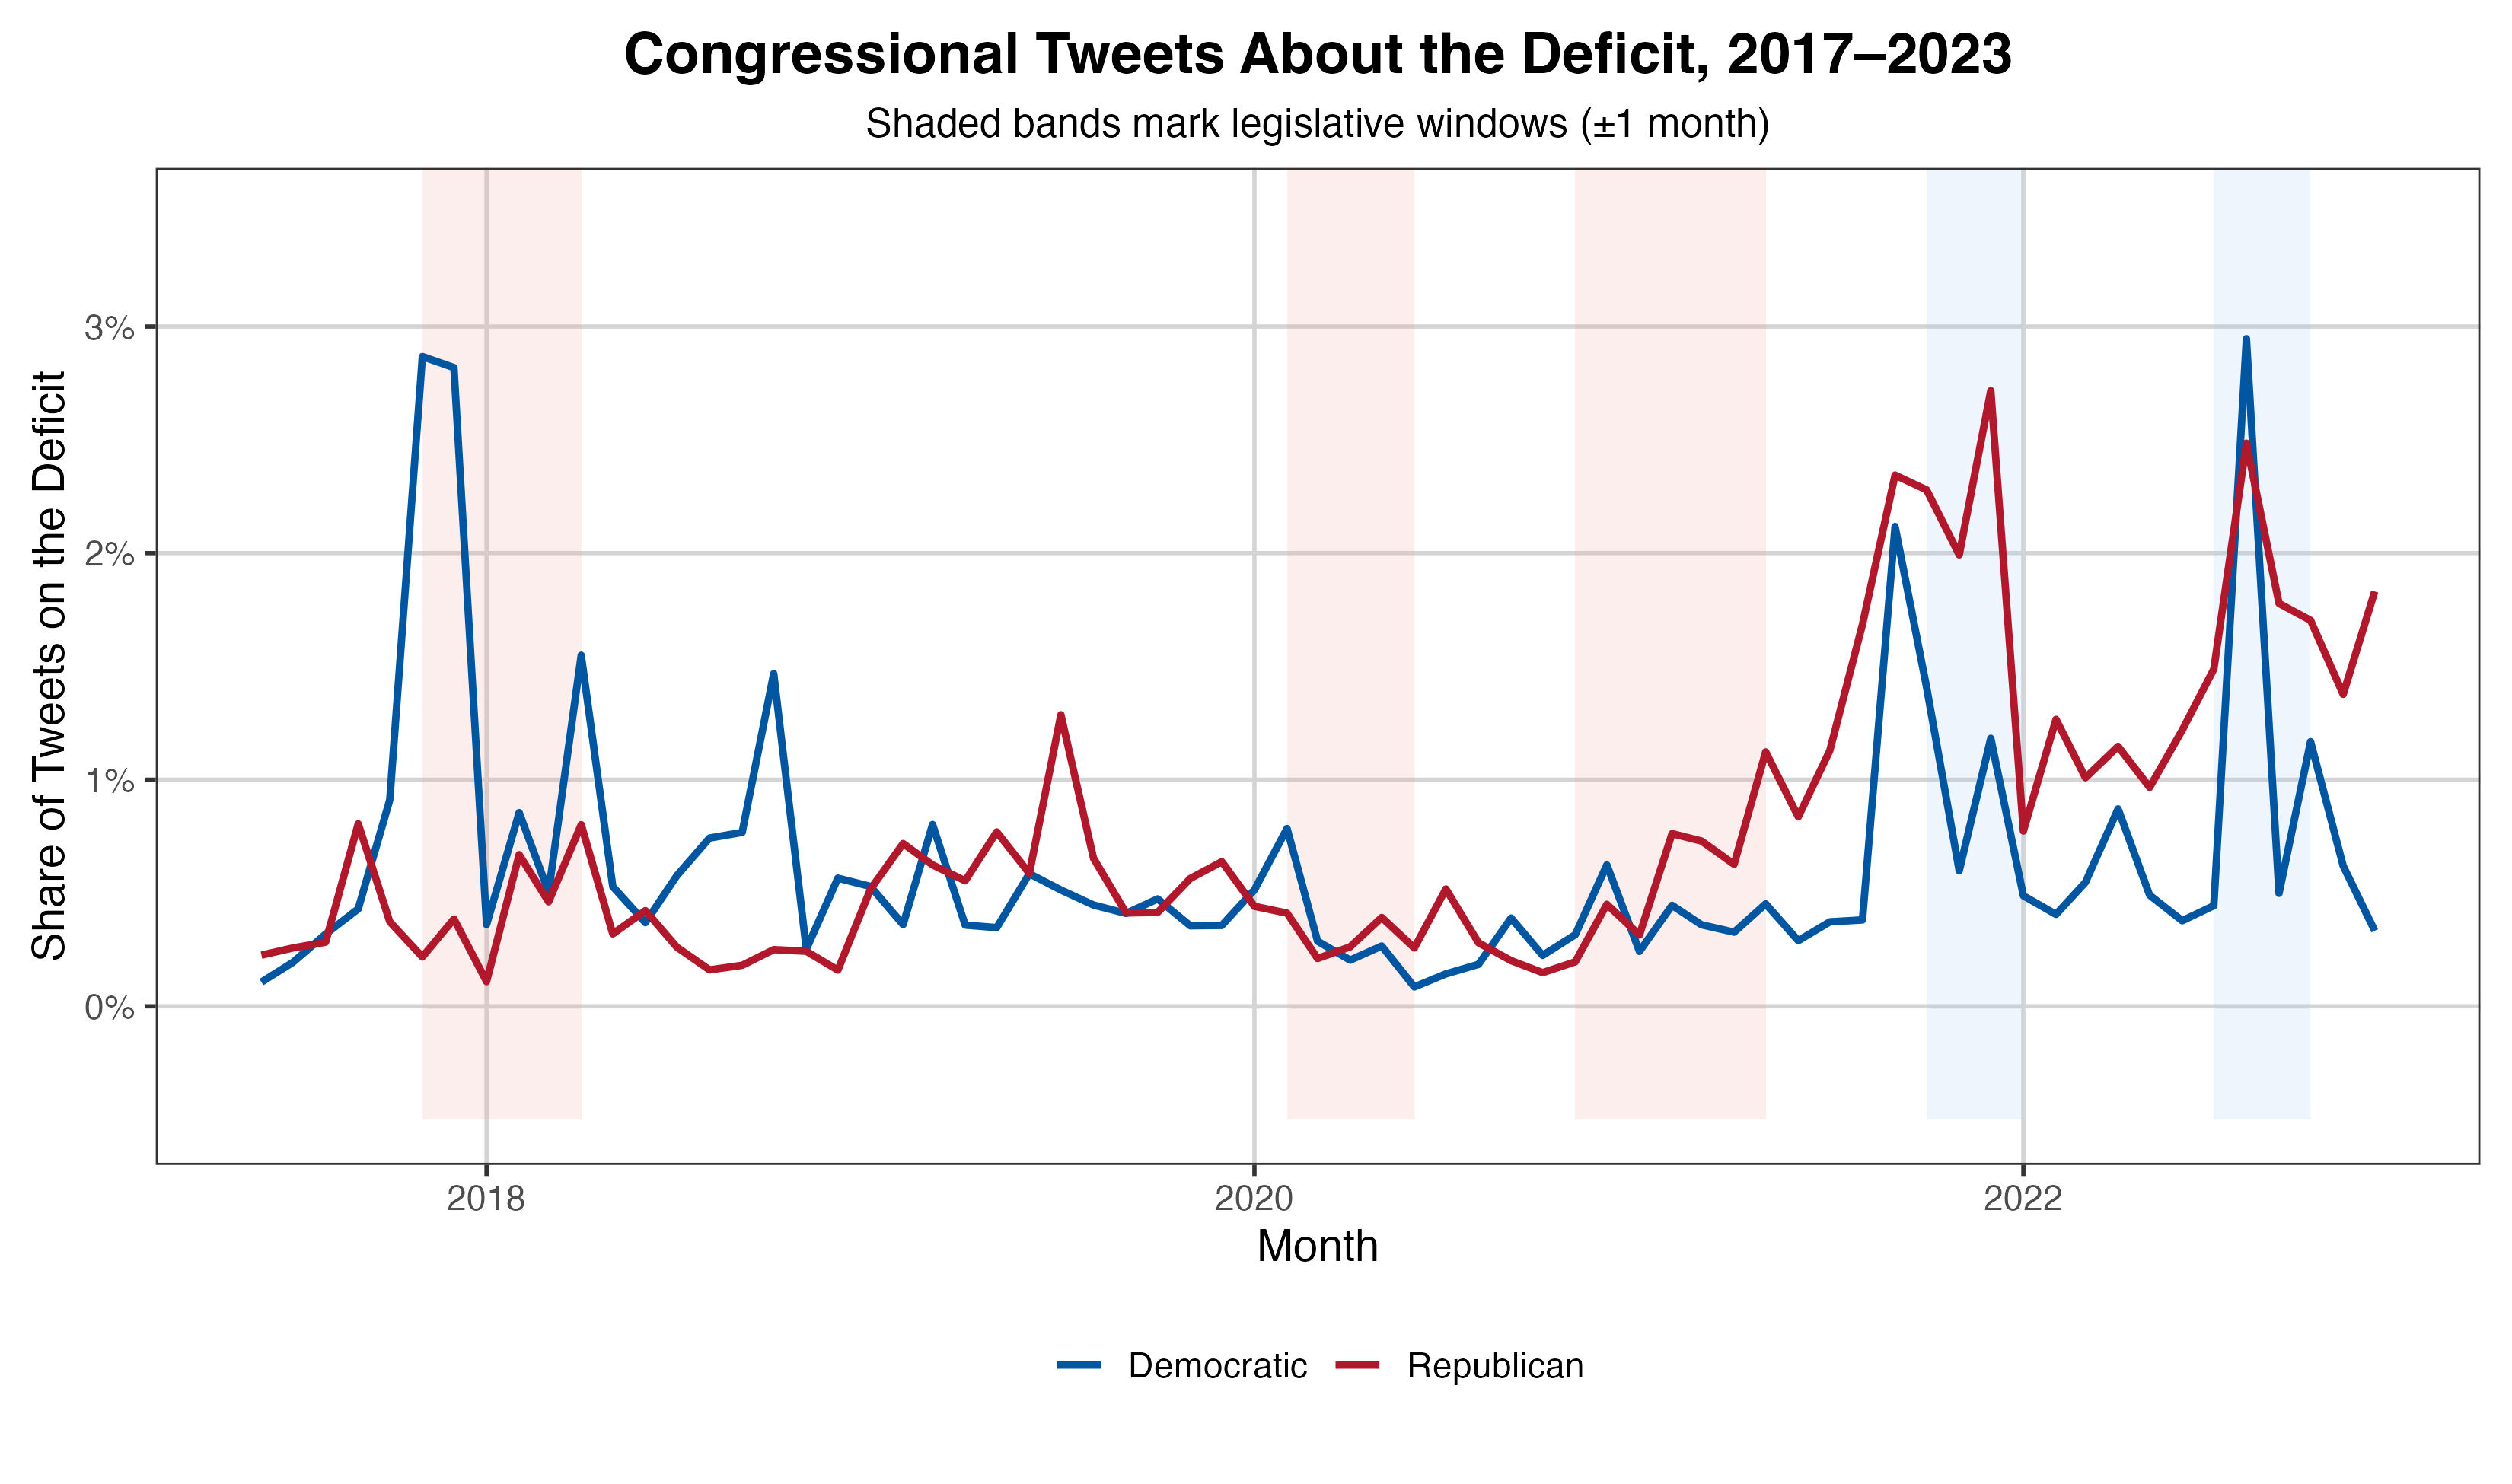
\includegraphics[width=0.85\linewidth,height=\textheight,keepaspectratio]{../figures/summary/deficit_tweet_share_with_legislation.png}

}

\caption{\label{fig-timeseries}Share of congressional tweets about the
deficit.}

\end{figure}%

The baseline deficit tweeting share for both parties is low, generally
under 1\% when averaged across members over six years, with notable
accelerations occurring around legislative periods. Democratic tweeting
patterns remain relatively consistent across the six years, with three
notable peaks, all during periods: December 2017 (Tax Cuts and Jobs
Act), October 2021 (Infrastructure Investment and Jobs Act), and August
2022 (Inflation Reduction Act, CHIPS \& Science Act). Republicans,
however, demonstrate consistently higher deficit tweeting rates as the
minority party, as illustrated in the peaks (2022, 2023) compared to
relatively low rates from 2017-2021.

\section{Economic Indicators}\label{economic-indicators}

Figure~\ref{fig-deficit-vs-cpi} plots deficit tweet share against US CPI
inflation (YoY) reveals a relatively strong positive relationship, as
indicated by its large r-value (.78). There are a few plausible
explanations for this linear relationship. First, the elevated inflation
rates of 2022, peaking at 9.1\% in June (40-year high), may have
increased elected officials concern about deficit spending. Public
discontent over higher prices may have also pressured representatives to
take a more hawkish approach on federal expenditures.

\begin{figure}[htbp]

\centering{


\includegraphics[width=0.8\linewidth,height=\textheight,keepaspectratio]{../figures/economic_indicators/deficit_share_vs_inflation_smoothed.png}

}

\caption{\label{fig-deficit-vs-cpi}Deficit tweet share vs.~U.S. CPI
inflation.}

\end{figure}%

Another explanation could be that along with higher inflation, the
significant fiscal legislation being proposed in the summer of 2022
(e.g, IRA, CHIPS) may have drawn concerns from representatives prompting
more congressional tweets on the topic.

\section{Member-Level Patterns}\label{member-level-patterns}

\begin{figure}[H]

\centering{

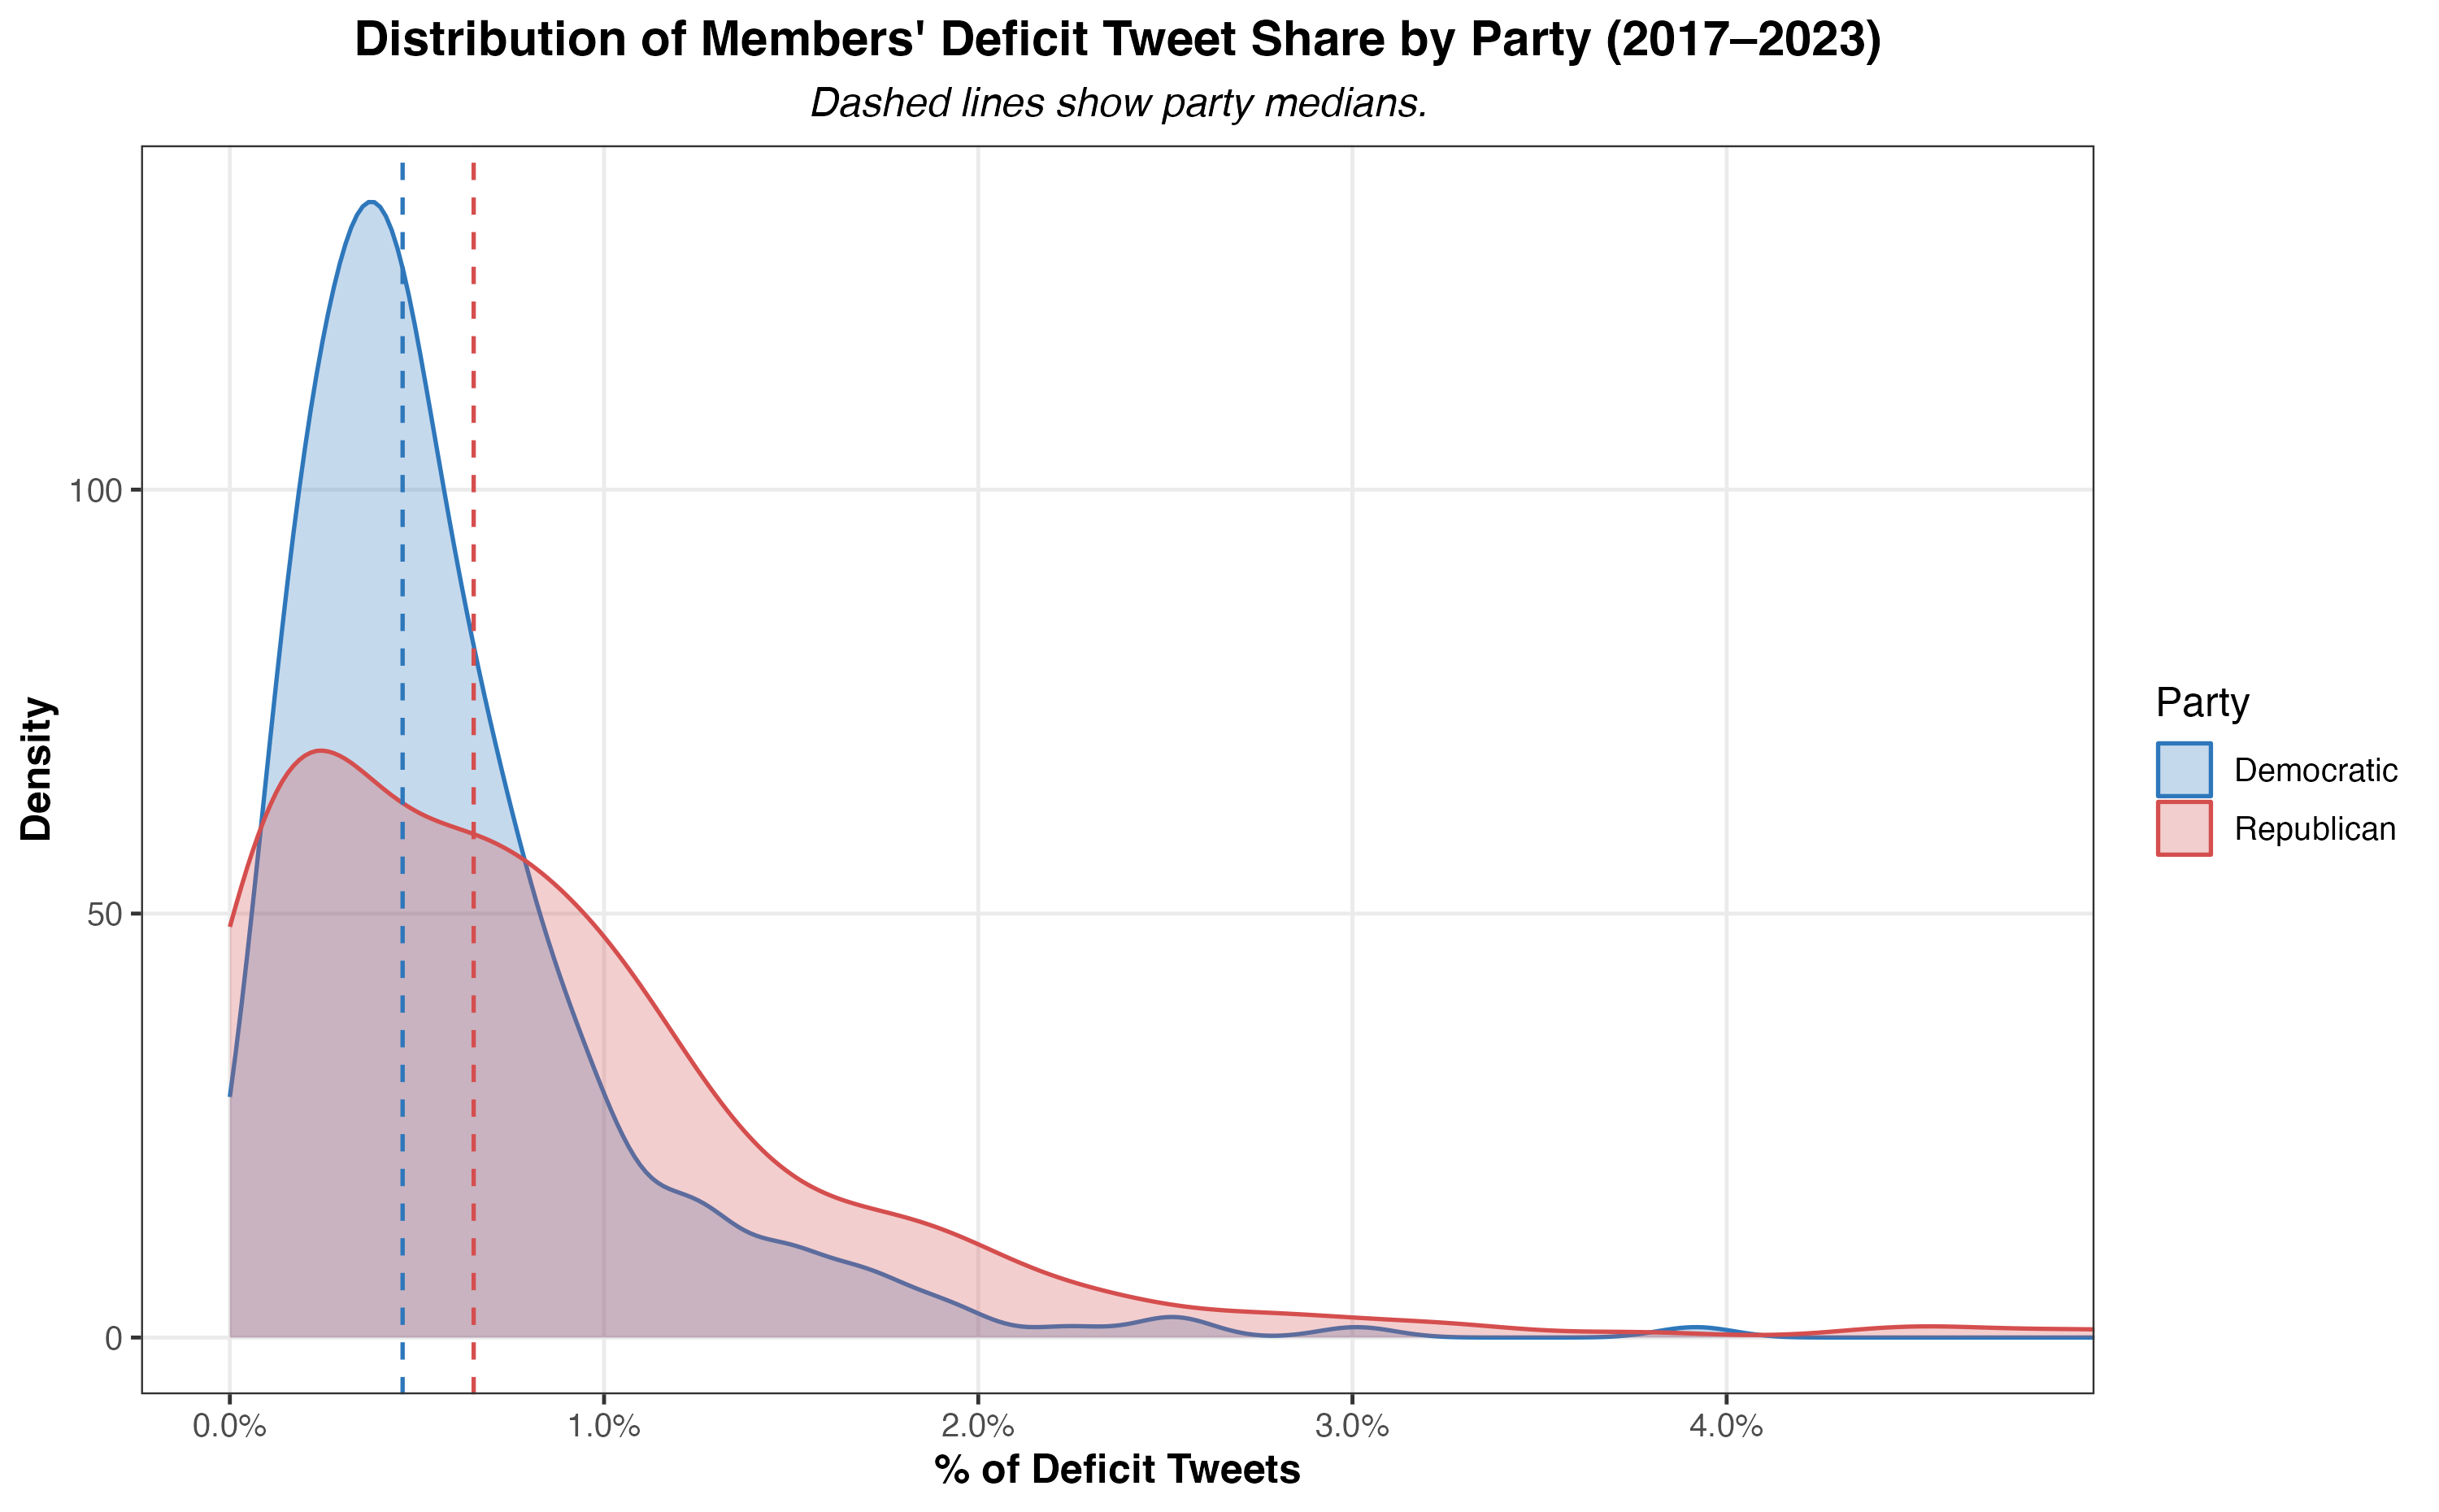
\includegraphics[width=0.8\linewidth,height=\textheight,keepaspectratio]{../figures/individuals/density_pct_deficit_by_party_overall.png}

}

\caption{\label{fig-member-share-by-party}Share of deficit tweets by
party (member-level distribution).}

\end{figure}%

Figure~\ref{fig-member-share-by-party} presents member-level
distributions of deficit tweeting, calculated as the share of each
member's tweets that mention the deficit over the entire period. As
illustrated by the dashed lines (party medians), Republicans tweet about
the deficit more frequently than Democrats, with average shares of
0.81\% and 0.62\%, respectively.

Democrats display a relatively compact distribution, with most
representatives falling below 0.7\%, indicating less intra-party
variation in deficit tweeting. Republicans, however, show far greater
variability within their party. The GOP's right tail distribution
illustrates that, compared to their Democratic colleagues, a far greater
proportion of members tweet about the deficit at much higher rates, with
outliers reaching 4--8\%.

Figure~\ref{fig-power-boxplot} breaks down these distributions further
by institutional power status (majority vs.~minority). The left and
right panels juxtapose the distribution when a member's party controls
the presidency (in-power) versus when it does not (out-of-power). For
instance, Democrats would be considered in-power from January 2021 to
January 2023 under President Joe Biden, while Republicans would be
out-of-power during this same period.

\begin{figure}[H]

\centering{

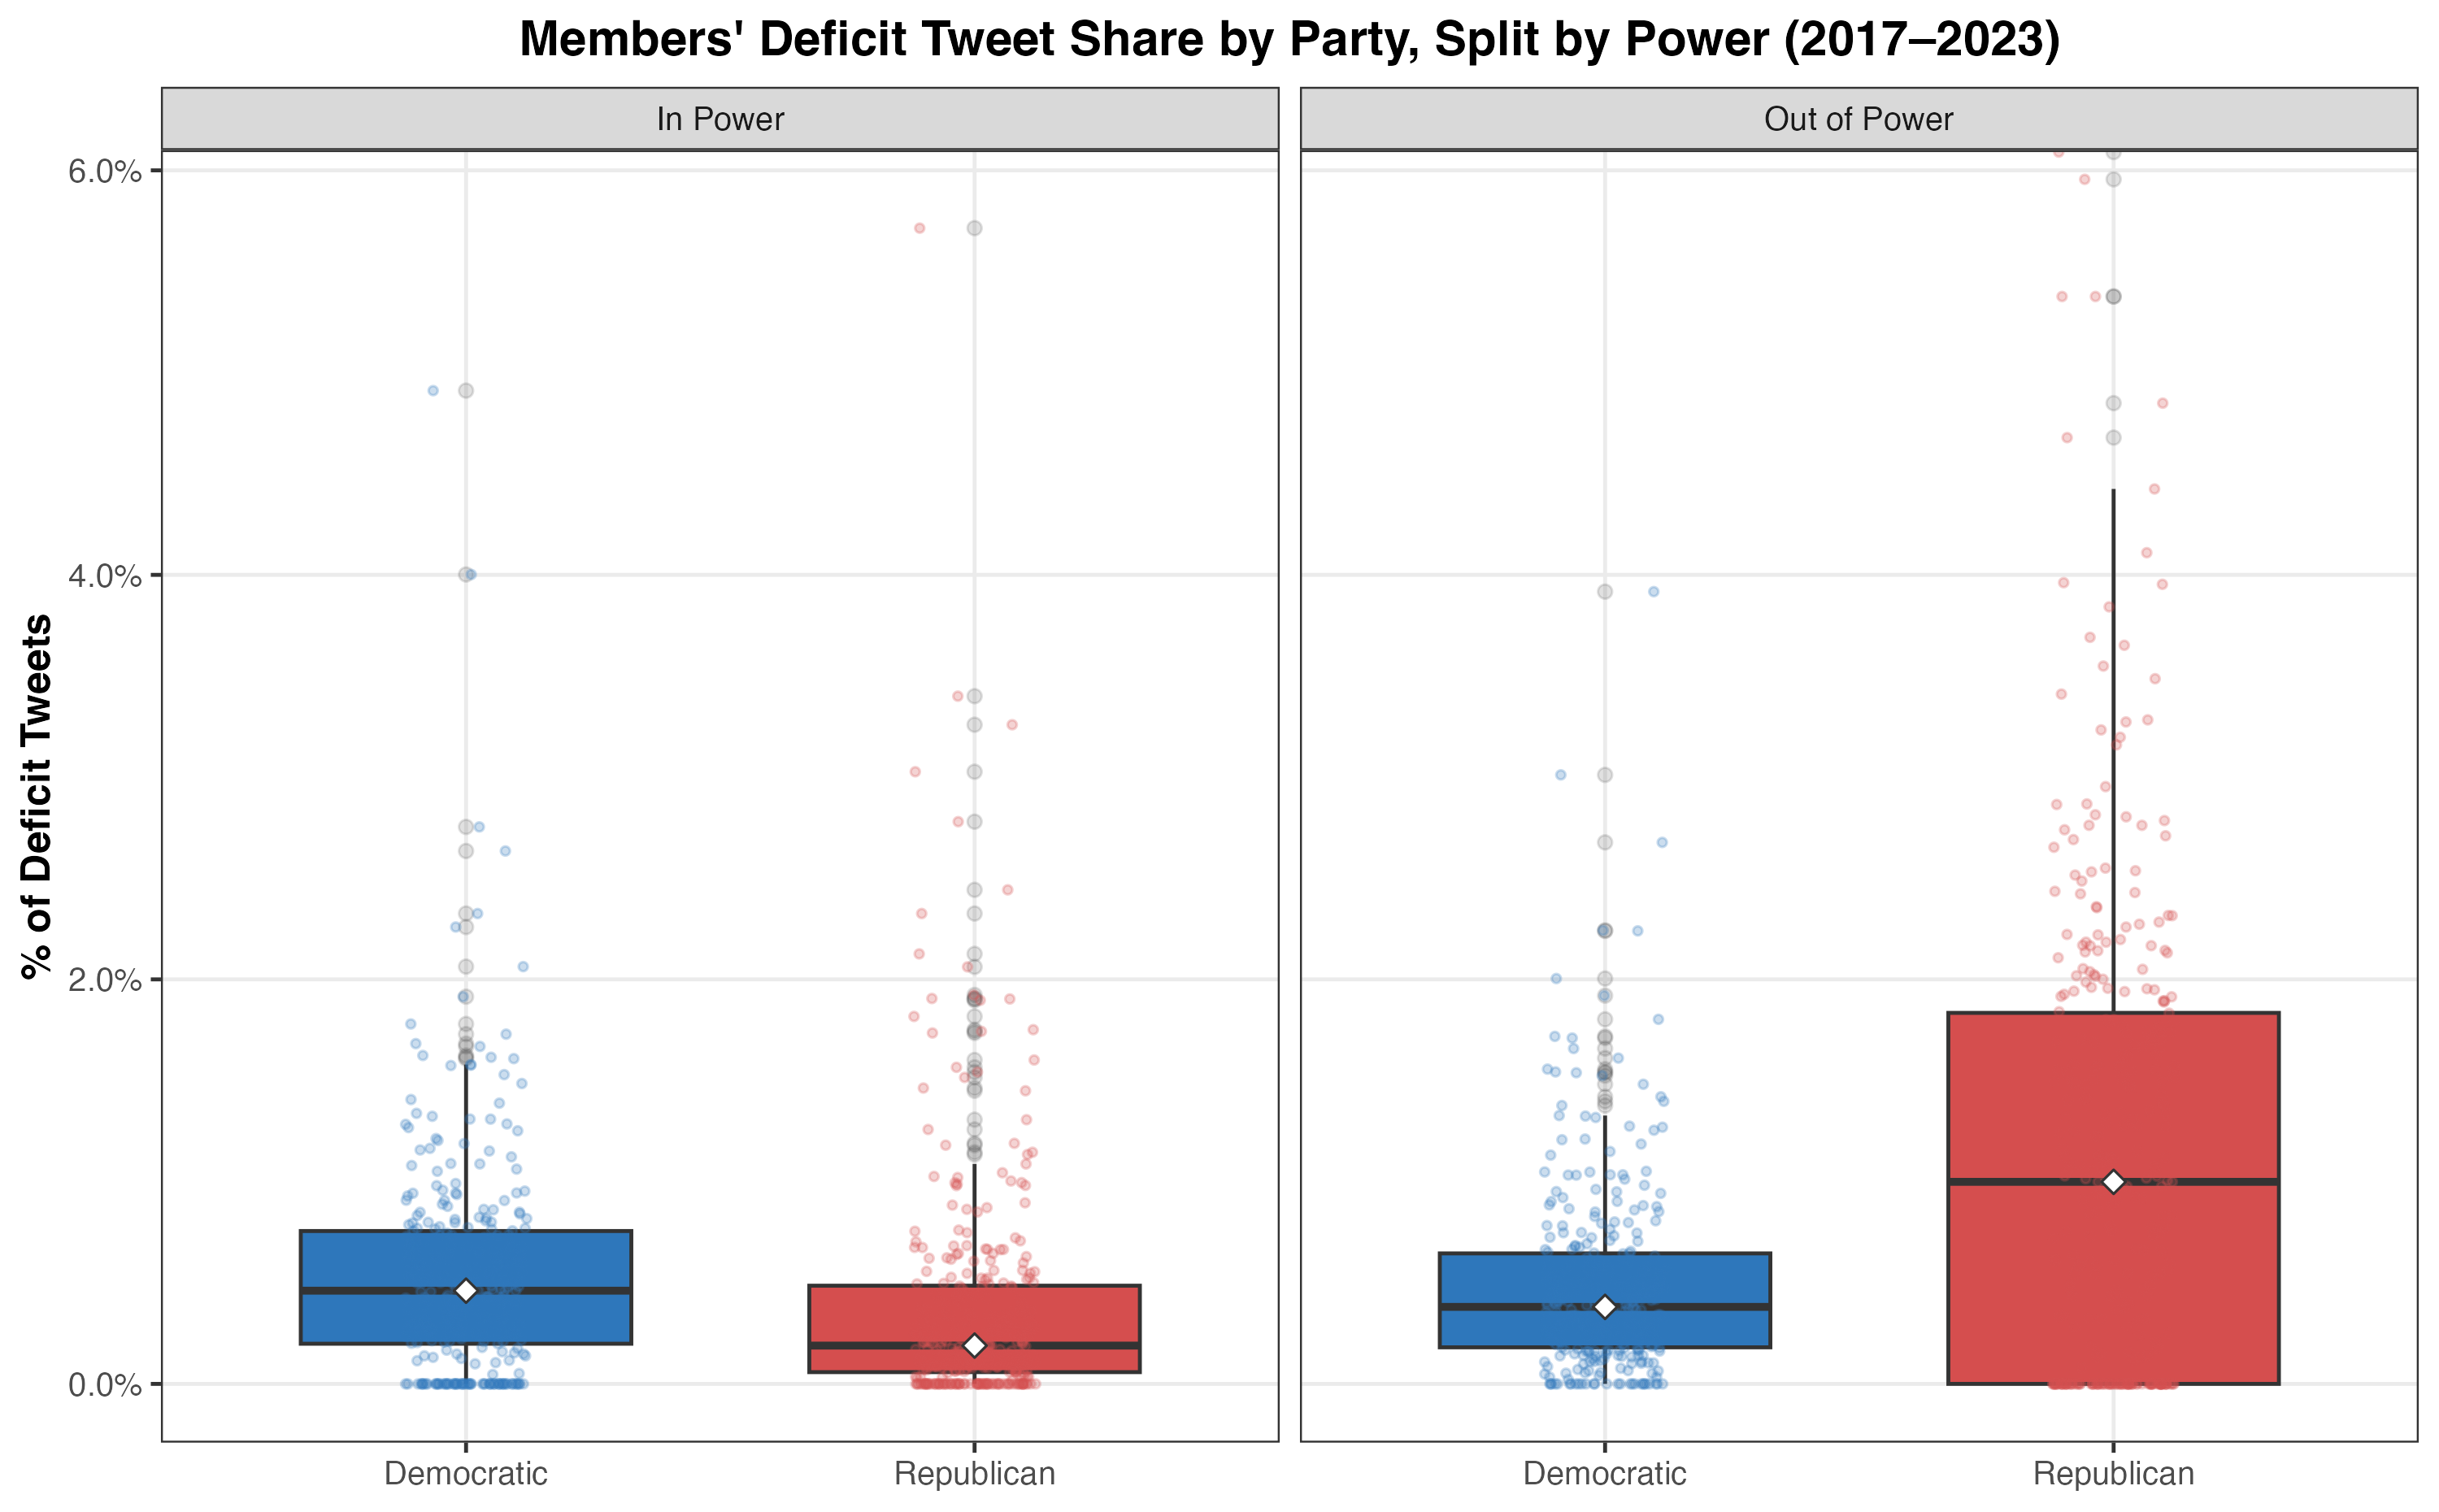
\includegraphics[width=0.8\linewidth,height=\textheight,keepaspectratio]{../figures/individuals/box_party_split_by_power.png}

}

\caption{\label{fig-power-boxplot}Distribution of deficit tweets by
power (boxplot).}

\end{figure}%

Figure~\ref{fig-power-boxplot} shows a clear asymmetry in GOP tweeting
patterns between these periods. When moving between power contexts, the
GOP median tweet share increases five-fold, from 0.2\% to 1.0\% and the
interquartile range from 0.6\% to 1.8\%. Put simply, Republicans were
far more likely to tweet about the deficit under President Biden than
under President Trump. This stark distributional contrast illustrates a
synchronized and cohesive shift in messaging among Republicans:
emphasize the deficit more in periods of political weakness. Democrats,
by contrast, remain relatively stable across contexts and actually
demonstrate a modest increase in spread and averages when in power.

\begin{figure}[H]

\centering{

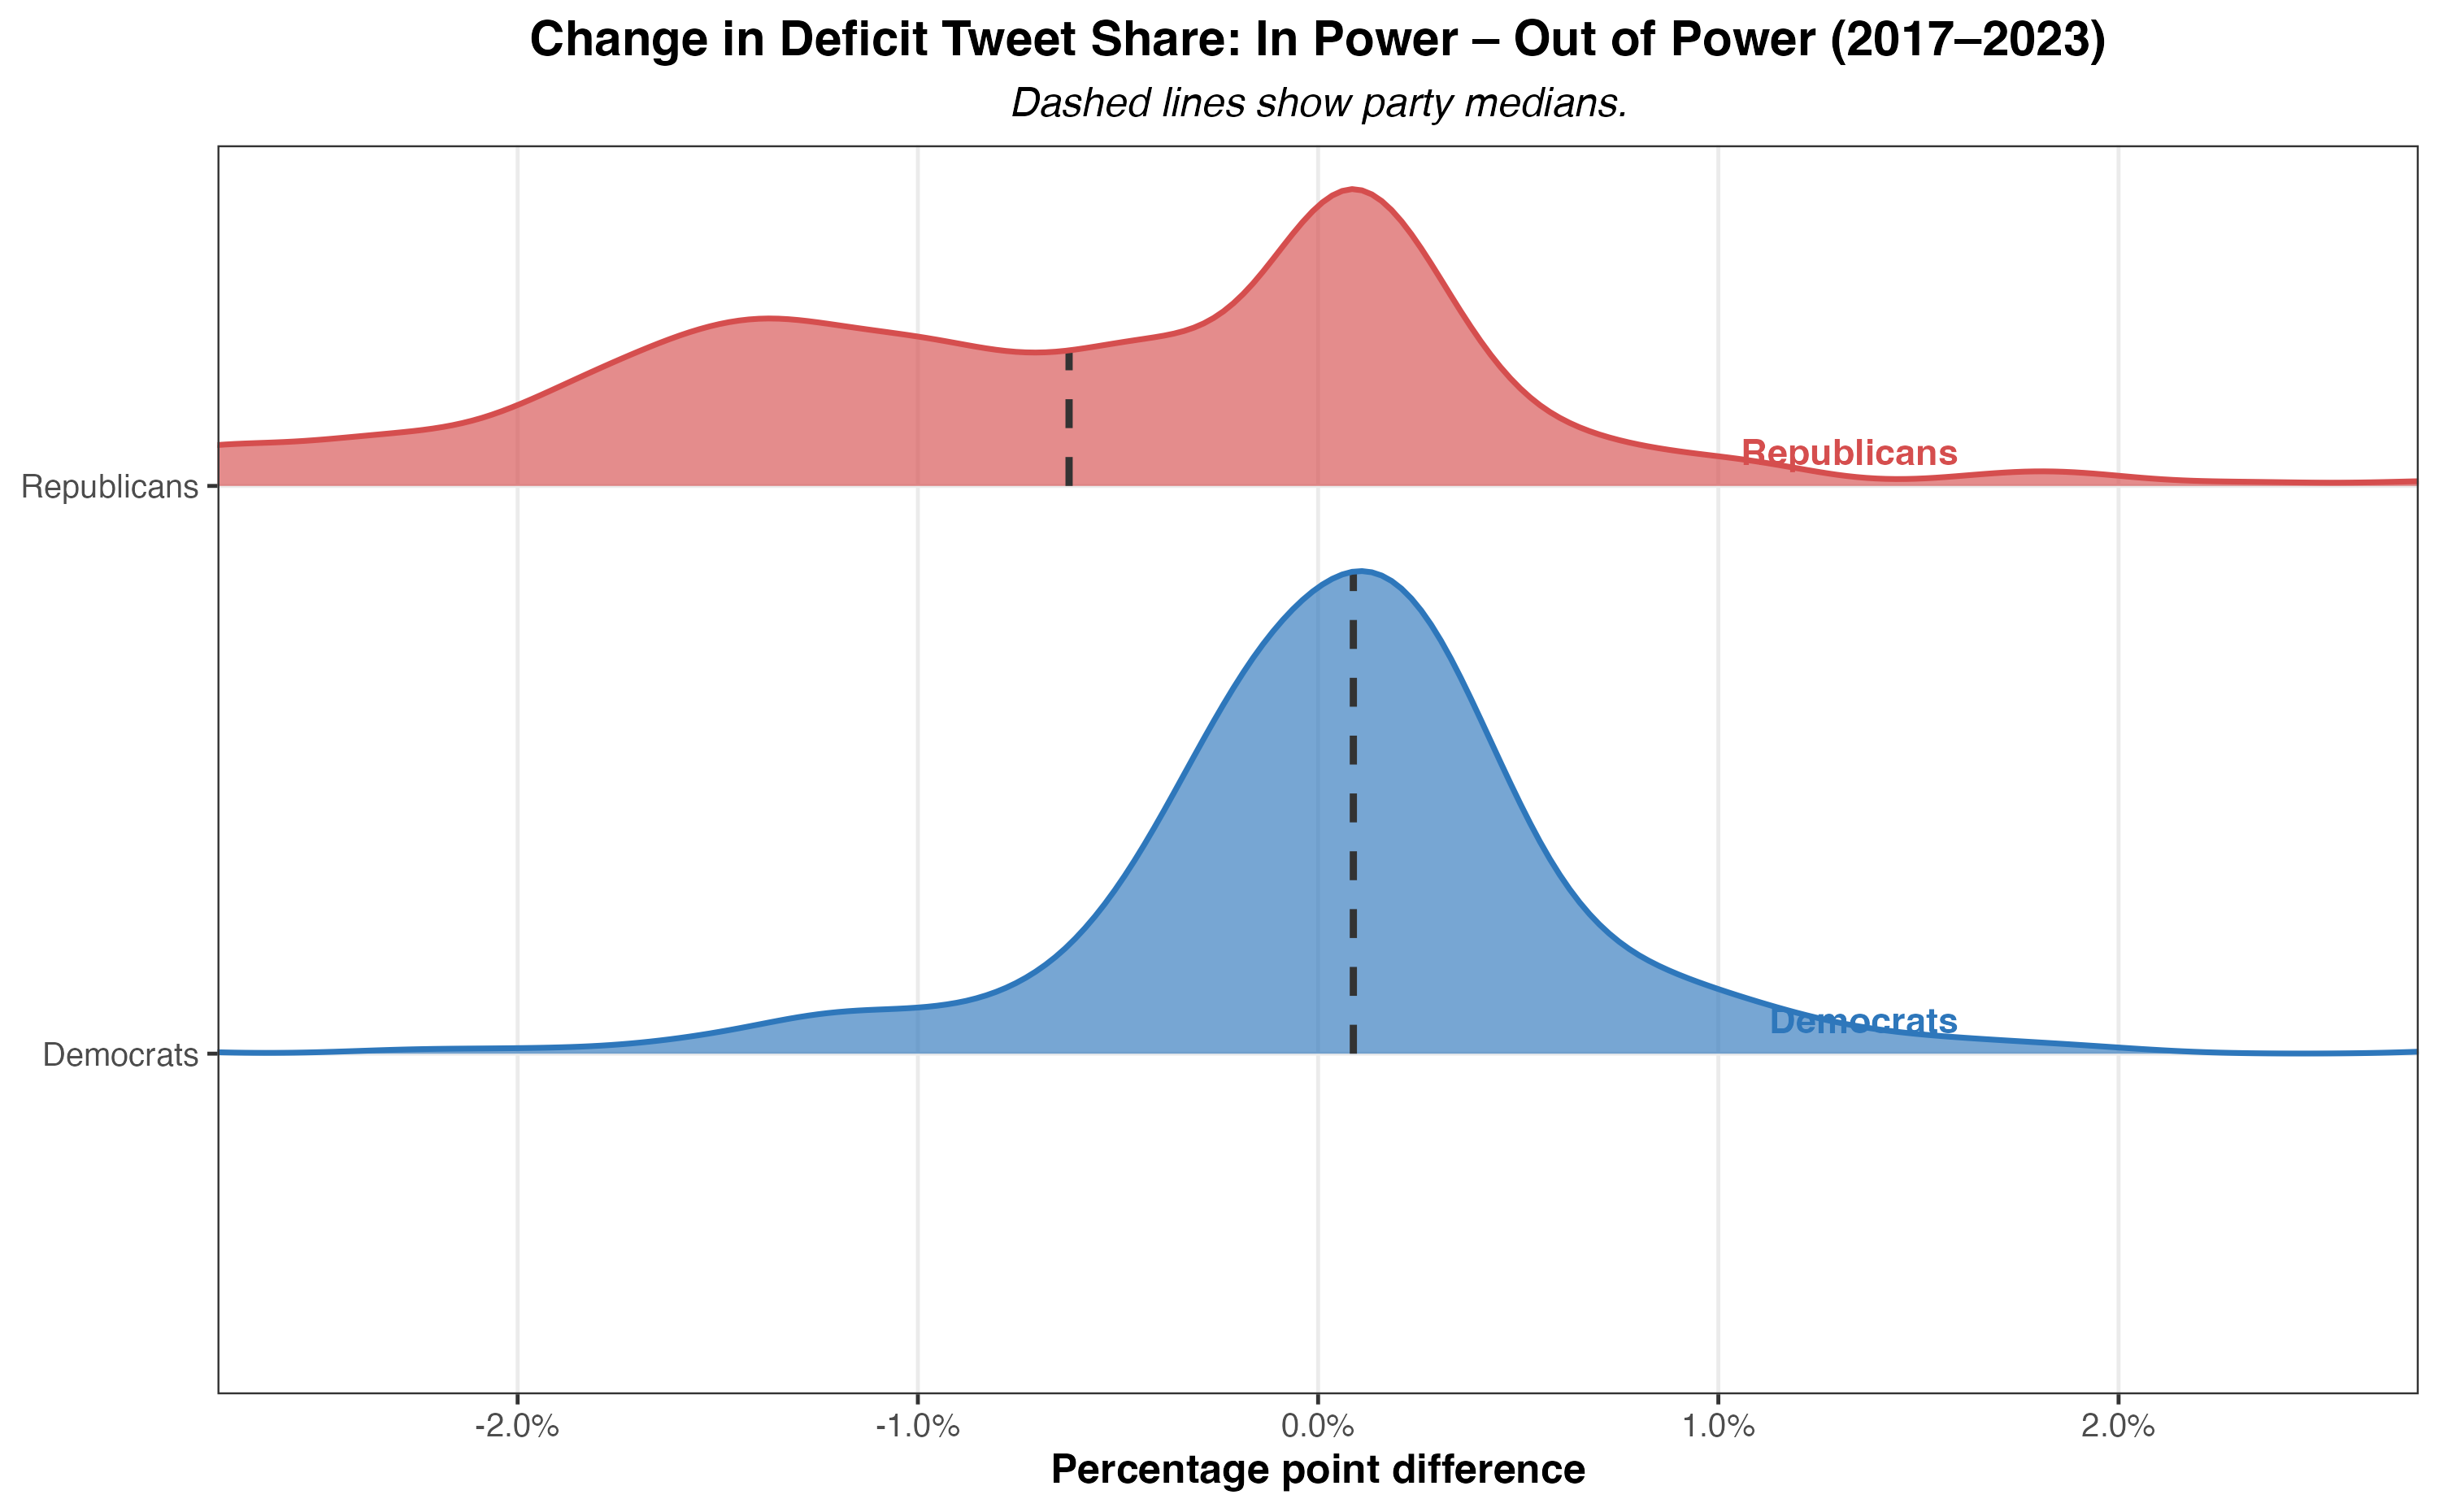
\includegraphics[width=0.8\linewidth,height=\textheight,keepaspectratio]{../figures/individuals/density_in_minus_out_overlay.png}

}

\caption{\label{fig-inout-shifts}In--out shifts in deficit tweeting
(histogram).}

\end{figure}%

Figure~\ref{fig-inout-shifts} visualizes these shifts more directly by
plotting the distribution of changes in deficit tweeting when moving
from in-power to out-of-power contexts. The x-axis represents the
difference in deficit tweet share between these two periods for each
member (in minus out). Positive values indicate that a member tweeted
more about the deficit when in power, while negative values indicate
higher tweeting rates when out of power. The GOP's comprehensive party
shift is evident, with the bulk of the party's distribution skewed
negative.

Taken together, Figure~\ref{fig-power-boxplot} and
Figure~\ref{fig-inout-shifts} suggest that Republicans are far more
sensitive to power status when deciding how frequently to tweet about
the deficit, while Democrats maintain a more consistent messaging
strategy regardless of institutional control. Furthermore, these results
illustrate a broader point about the degree of strategic messaging
coordination among parties. The pronounced and systematic increase in
Republican deficit tweeting supports the notion of uniform, top-down
messaging within the party. Democrats, by contrast, show less cohesion
in their messaging strategy, with members displaying a wider range of
tweeting behaviors across power contexts.

\section{Leadership Analysis}\label{leadership-analysis}

Figure~\ref{fig-leadership} summarizes deficit-tweeting by House and
Senate leaders across majority/minority contexts. Patterns differ by
party and chamber, with the sharpest contrasts in the Senate: Senator
Chuck Schumer tweeted about deficits far more as Majority Leader (4.0\%)
than as Minority Leader (1.0\%), while Senator Mitch McConnell did the
reverse (1.9\% in the minority vs.~0.05\% in the majority). In the
House, Representative Pelosi tweeted about deficits more in the minority
(1.1\%) than as Speaker (0.5\%).

\begin{figure}

\centering{


\includegraphics[width=0.85\linewidth,height=\textheight,keepaspectratio]{../figures/leadership/leader_deficit_tweets.png}

}

\caption{\label{fig-leadership}Deficit tweeting by congressional leaders
(House and Senate; majority vs.~minority roles).}

\end{figure}%

Notably, Representative McCarthy ``has relatively few tweets (n = 762).
Because leaders often switch or add handles when roles change, the data
collection process may have failed to include relevant accounts.Thus,
McCarthy's deficit tweet share should be interpreted cautiously.

Taken together, these patterns illustrate that deficit rhetoric among
congressional leaders varies systematically with institutional role and
party, mirroring---and in some cases, amplifying---the broader
party-level trends documented above.

While preceding analysis covers broader party-level trends, exploring
individual leaders' tweeting patterns provides us insight into how key
political figures communicate about the deficit in varying institutional
contexts. Considering the legislative and electoral significance of
these figures, their messaging strategies are more influential and
calculated than rank-and-file members. For instance, party leaders may
use specific communication strategies around legislative periods to
catalyze or bar the passage of key bills.Thus, examining these trends
can help illustrate the degree of strategic communication employed by
top legislators, and by extension - the party they represent.

For instance, Representative Paul Ryan - a self-described fiscal
conservative and Speaker (2017-2019) - is a central political figure in
modern discourse surrounding the national deficit. While Ryan frequently
branded himself a ``deficit hawk,'' his public messaging during unified
GOP control downplayed the deficit as Congress advanced the Tax Cuts and
Jobs Act, which the CBO estimated would add roughly \$1.5 trillion to
the debt over ten years. In short, Ryan rarely emphasized the deficit
while orchestrating a major deficit-increasing legislative agenda.

Aside from highlighting rhetorical patterns in key legislators,
Figure~\ref{fig-leadership} also underscores a broader point about
communication uniformity among party leaders and rank-and-file
representatives. Previous research establishes the growing polarization
in congressional ideology and party-line voting (CQ Roll Call 2024). My
research provides insight into the specific polarities of a single
rhetorical subject---the federal deficit. For Democrats, the divergent
tweeting patterns of Speaker Pelosi and Senator Schumer suggest a
comparatively weaker intra-party alignment in messaging. These patterns
are consistent with the broader Democratic caucus, which shows no
discernible difference in deficit tweeting between power contexts (as
shown in Figure~\ref{fig-power-boxplot} and
Figure~\ref{fig-inout-shifts}).

The GOP, however, presents a more uniform party dynamic. Senator
McConnell's increase in deficit tweeting in out-of-power contexts
mirrors the broader Republican trend illustrated in
Figure~\ref{fig-inout-shifts}. Furthermore, McConnell's tweeting
patterns confirm long-held conceptions about his communication and
political style, which emphasizes unrelenting opposition to Democratic
fiscal policies.

The two messaging strategies employed by party leaders reflect a broader
division in party dynamics between Democrats and the GOP. These results
provide nuance to our understanding of the communication strategies of
key political figures, such as Representative Ryan and Senator
McConnell, whose ``deficit'' messaging has had significant implications
for historical and contemporary American fiscal policy.

\section{Legislative Context}\label{legislative-context}

\begin{figure}[htbp]

\centering{

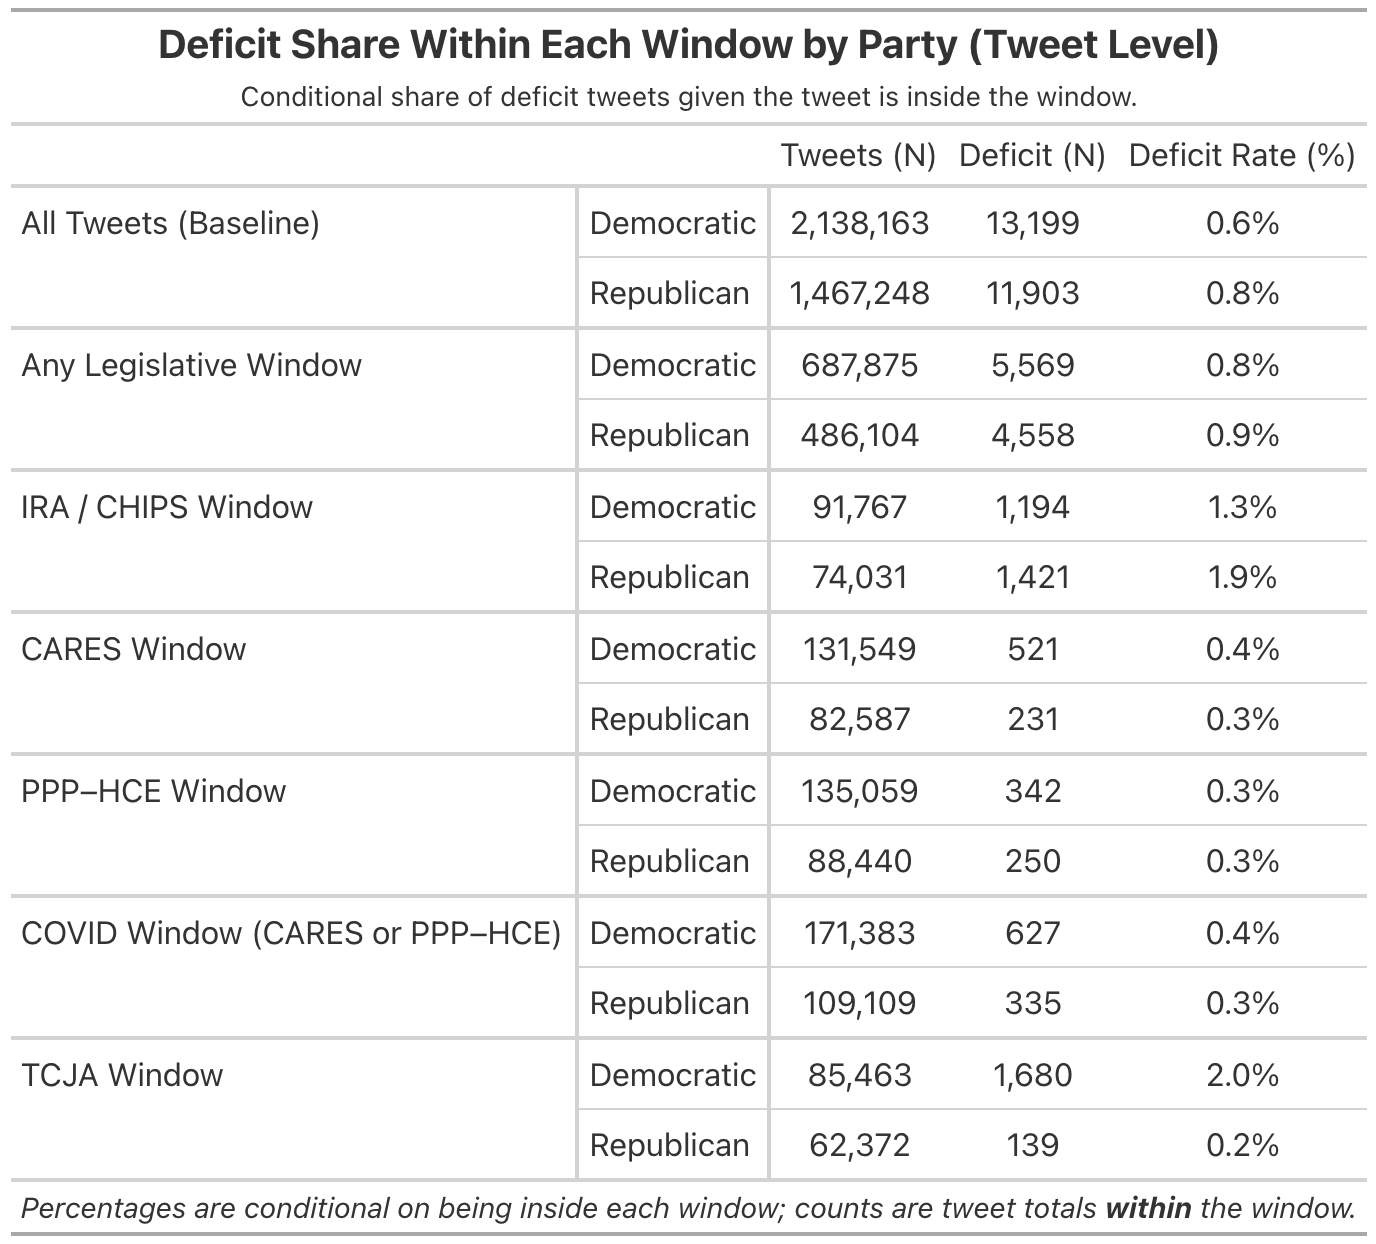
\includegraphics[width=0.75\linewidth,height=\textheight,keepaspectratio]{../results/good_summary_tables/tweetlevel_deficit_share_by_party.png}

}

\caption{\label{fig-deficit-share-by-party}Deficit share within
legislative windows, by party.}

\end{figure}%

Figure~\ref{fig-deficit-share-by-party} reports the conditional share of
tweets mentioning the deficit within ±1-month windows around major
bills, split by party (with a pooled/overall column for reference). At
baseline, Republicans tweet about the deficit more often 0.8\% than
Democrats 0.6\% -- a gap that persists across most legislative windows.
During the Inflation Reduction Act (2022) and CHIPS Act (2022) periods,
Republicans' tweets accelerated, with deficit mentions at nearly 2.0\%,
compared to 1.3\% among Democrats. However, the TCJA (2017)---a partisan
GOP tax cut---is a noticeable and stark exception. During these three
months, the Democrats' deficit share spikes to 2.0\%, while the
Republicans' share falls to just 0.2\%, reflecting a partisan
realignment around a highly divisive bill. In contrast, during the COVID
relief period in 2020 -- a non-partisan voting context -- both parties
converged at very low levels (0.3--0.4\%).

\section{Regression Visualization}\label{regression-visualization}

The following regression models offer a structured approach to examining
how institutional, fiscal, and partisan contexts affect the likelihood
of congressional deficit tweeting.

Since the specifications rely heavily on interaction terms, it is useful
to provide a framework for their interpretation first. The coefficients
are expressed as odds ratios: values above one indicate that Republicans
are more likely to tweet about deficits relative to Democrats. In
contrast, values below one indicate a narrowing of the GOP-Dem gap. Each
model includes majority interaction coefficients of the general form GOP
× Conditioning Variable. These coefficients indicate whether the baseline
Republican--Democratic difference changes under specific conditions
(legislative windows, presidential control, chamber control, or
trifectas).

\begin{figure}[htbp]

\centering{

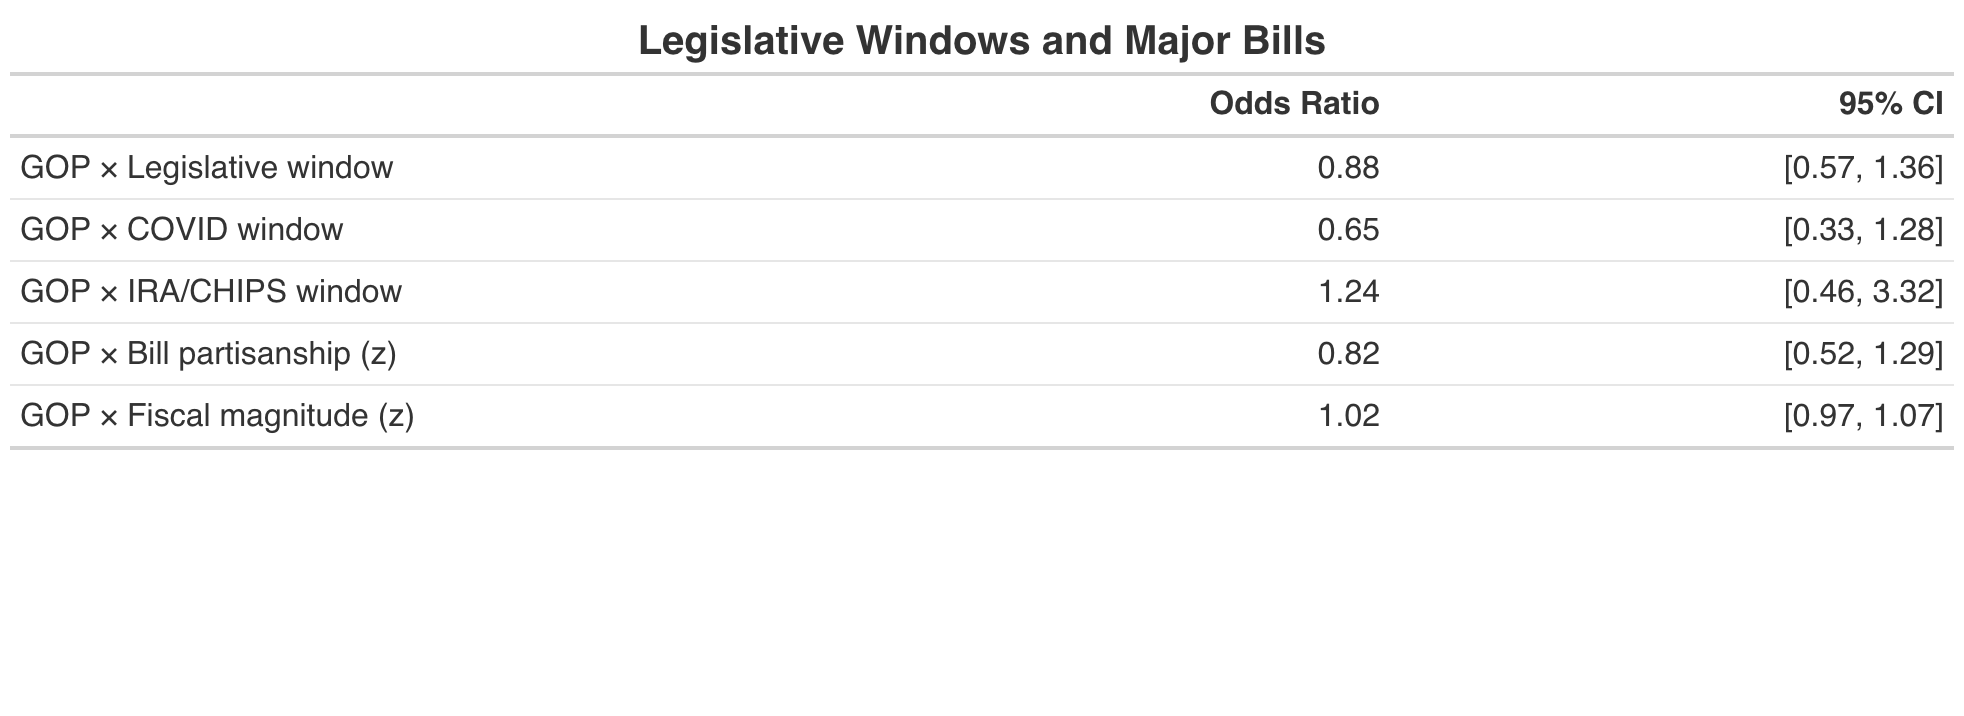
\includegraphics[width=0.75\linewidth,height=\textheight,keepaspectratio]{../results/good_regression_tables/r3_legislative_windows_main.png}

}

\caption{\label{fig-r1-legislative-windows}Regression 1: Legislative
windows.}

\end{figure}%

The baseline model, Figure~\ref{fig-r1-legislative-windows}, examines
partisan differences in legislative periods without conditioning on
institutional control. The non-significant results suggest that, when
averaged across both Democratic and Republican presidencies, legislative
windows themselves do not systematically impact the partisan gap in
deficit tweeting.

\begin{figure}[htbp]

\centering{

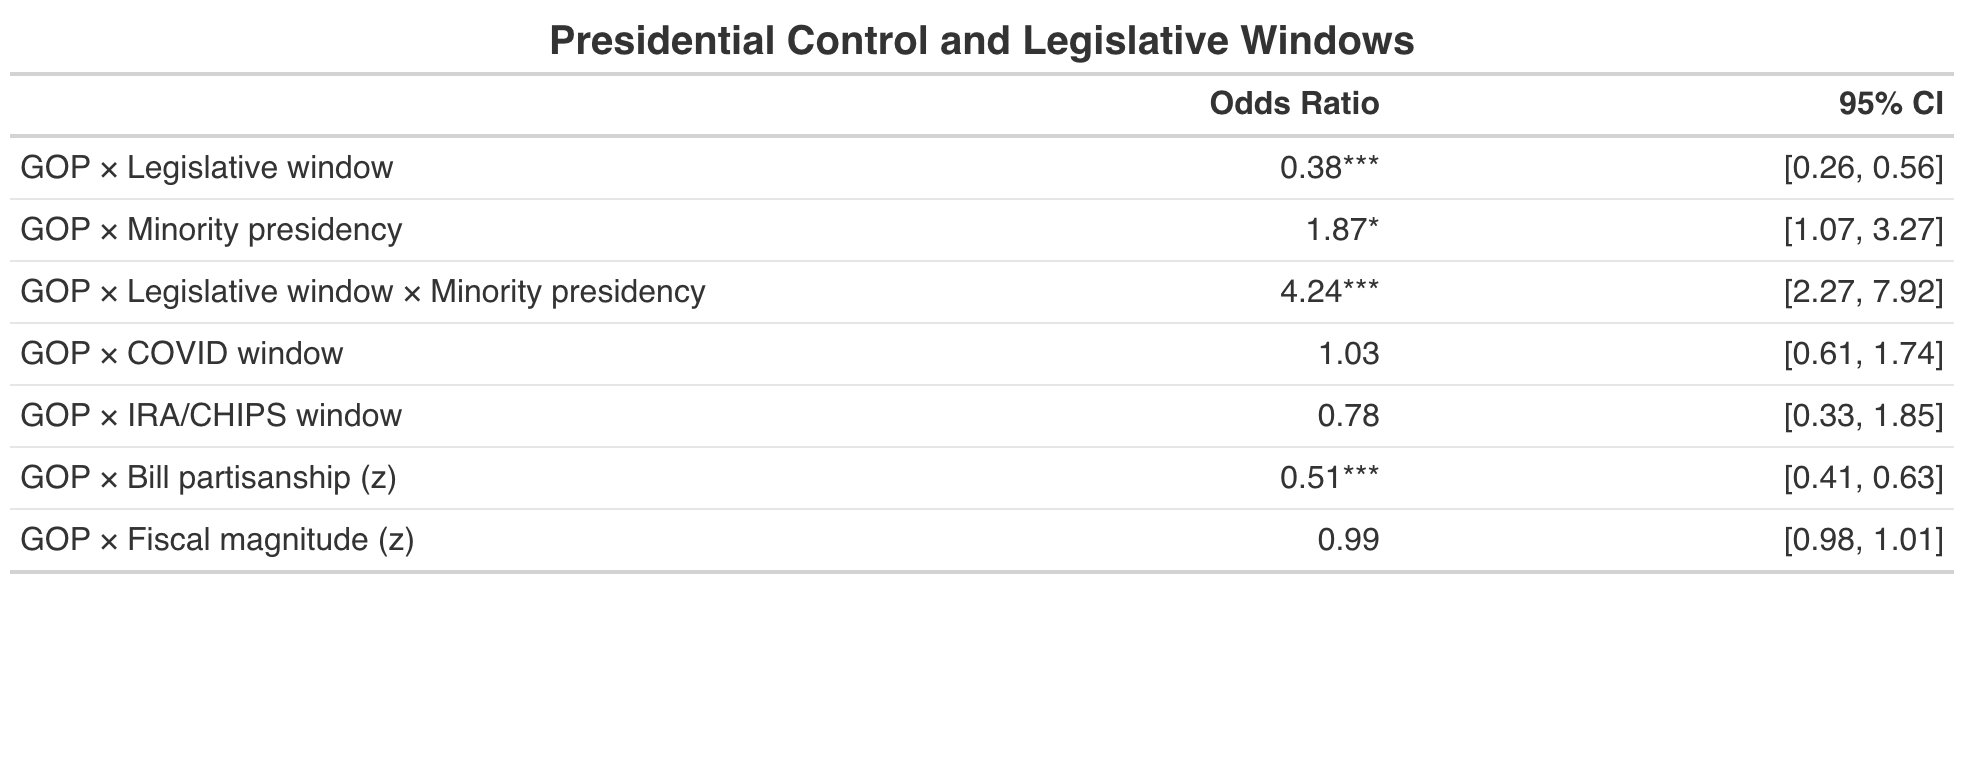
\includegraphics[width=0.75\linewidth,height=\textheight,keepaspectratio]{../results/good_regression_tables/r5_majority_context_main.png}

}

\caption{\label{fig-r2-presidency}Regression 2: Majority context
(presidency).}

\end{figure}%

Figure~\ref{fig-r2-presidency} controls for presidential party by adding
an indicator for servingunder the out-party president (GOP under a
Democratic president; Democrats under a Republican president)and by
interacting it with Legislative window, plus the three-way term GOP ×
Legislative window × Minority presidency. These terms let the GOP--Dem
deficit-tweeting gap differ under Democratic vs.~Republican presidents
and specifically during legislative months.

Republicans' odds of tweeting about deficits are nearly double (OR =
1.87) when not holding the presidency (i.e, Joe Biden is President)
compared to Democrats under the same condition. In contrast, GOP ×
Legislative window (OR= 0.38) highlights that under a Republican
presidency, the partisan gap narrows during legislative months---the
odds of the GOP tweeting are 62\% lower than those of Democrats. This
pattern aligns with Figure 1, which shows that Republican tweeting
contracts while Democratic tweeting spikes as Congress passes the Tax
Cuts and Jobs Act in late 2017. However, the three-way interaction
coefficient GOP × Legislative window × Minority presidency reveals a
reversal of this trend (OR= 4.24). Under a Democratic presidency (Joe
Biden), Republicans' odds of tweeting are more than four times higher
than those of Democrats in the same condition.

\begin{figure}[htbp]

\centering{

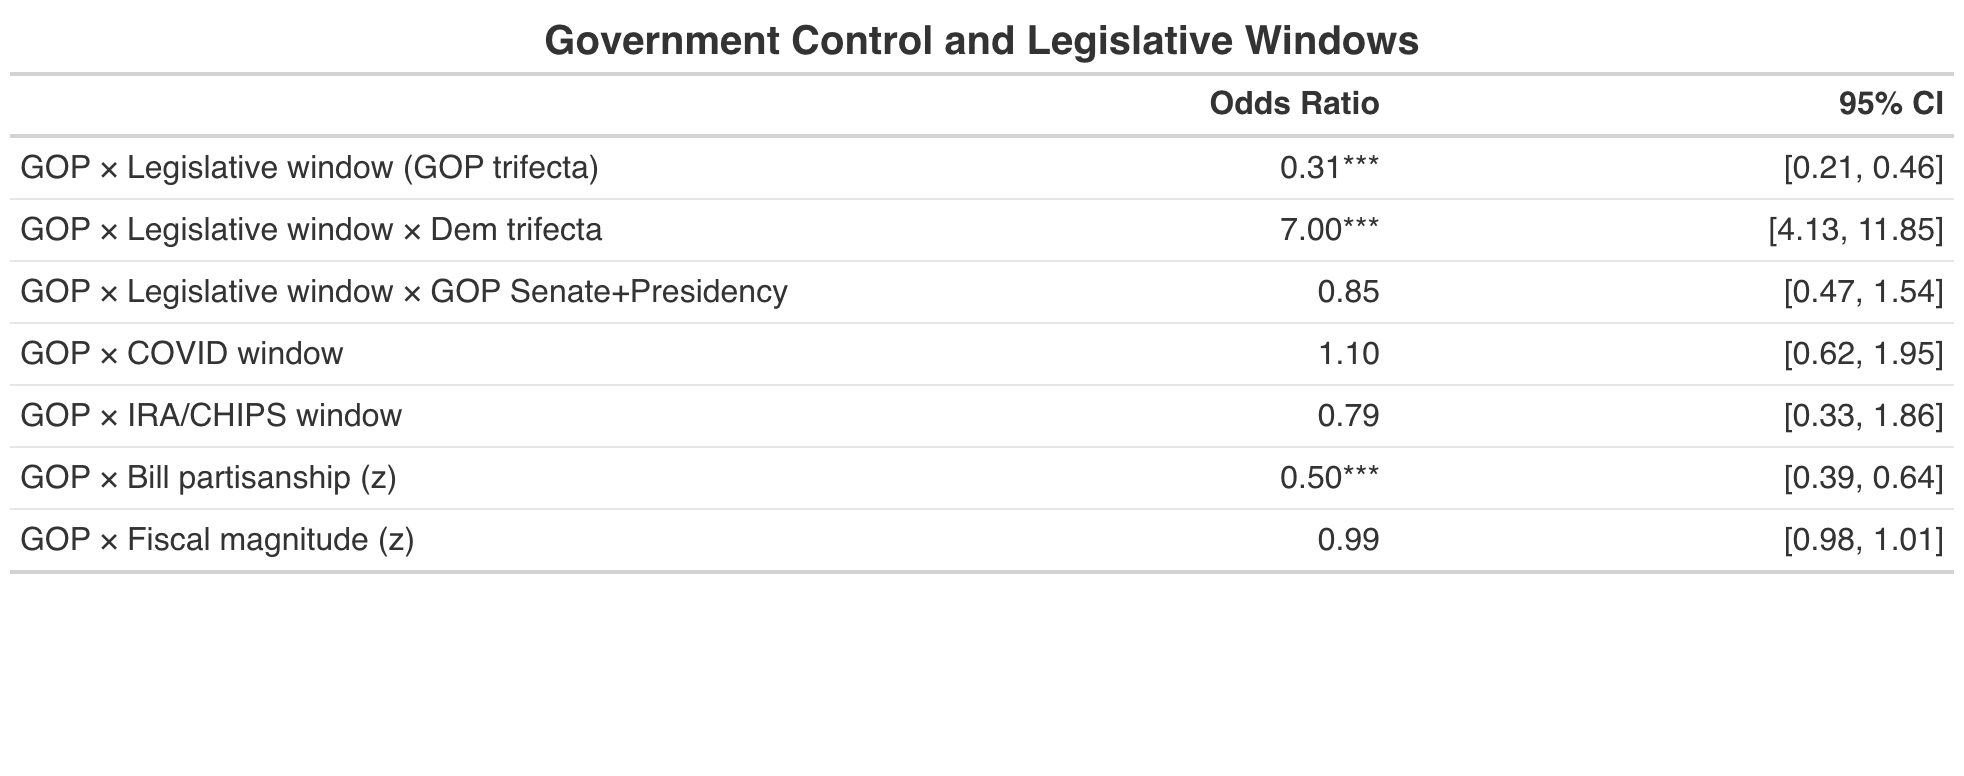
\includegraphics[width=0.75\linewidth,height=\textheight,keepaspectratio]{../results/good_regression_tables/r6_majority_context_combos.png}

}

\caption{\label{fig-r3-chamber-presidency}Regression 3: Majority context
--- chamber and presidency combinations.}

\end{figure}%

Figure~\ref{fig-r3-chamber-presidency} examines how the tweeting gap
changes by who controls congressional and executive branches. A GOP
trifecta means Republicans held the presidency, House, and Senate
simultaneously---a condition they held from 2017 to 2019 during the
115th congress. The model includes indicators for these control
combinations: the baseline is Democrats outside legislative windows when
their party controls no institution (minority in both chambers and not
holding the presidency).Put differently, Democrats, between 2017 and
2019, in non-legislative periods (i.e, not during Tax Cuts andJobs Act).

GOP x Legislative window (OR = 0.31) indicates that during legislative
months, when holding a triecta, Republicans' odds of tweeting are 69\%
lower than Democrats. The Tax Cuts and Jobs Act (2017) -- a legislative
window under a GOP trifecta -- is an illustration of this condition.
However, once we condition on a Democratic trifecta, this effect
reverses. Relative to the baseline condition (a GOP trifecta),
Republicans' odds of deficit tweeting are seven times higher than those
of Democrats in the same context. The juxtaposition of these two
coefficients (OR = 0.31) versus (OR = 7.00) illustrates that legislative
timing by itself isn't a determinate of tweeting gaps---but who governs
is. Under Democratic control (i.e., 2021-2023), Republicans accelerate
deficit rhetoric during legislative months, while under the GOP trifecta
(i.e., 2017-2019), they significantly reduce deficit tweeting
frequencies.

\subsection{\texorpdfstring{\textbf{Bill Partisanship and Fiscal
Magnitude}}{Bill Partisanship and Fiscal Magnitude}}\label{bill-partisanship-and-fiscal-magnitude}

Across all three specifications, the coefficients for Fiscal magnitude
(z) remain consistently insignificant (\textasciitilde1.0).~ These
coefficients, based on a normalized measure of a given bill's 10-year
CBO estimate, suggest that the fiscal consequences of policy do not
systematically impact partisan tweeting gaps.

Bill partisanship (z), however, shows significant contractions in the
GOP-Dem tweeting gap once institutional control is included \textbf{(OR
\textasciitilde{} 0.50)}. In other words, for each one-SD increase in a
bill's partisanship score, the GOP-Dem gap contracts by roughly half.
Notably, because these variables are continuous (ie, z-scores), the
coefficients represent slopes rather than a baseline-specific effect.
For example, in the context of bill partisanship, if Republicans are
twice as likely as Democrats to tweet at \textbf{z = 0 (OR = 2.0)}, that
gap narrows to parity at \textbf{z = 1 (OR = 1.0).}

\FloatBarrier




\end{document}
